% Library Management System - Detailed Report
% Author: Piyush Raj Singh
% Date: November 3, 2025
\documentclass[12pt,a4paper]{article}
\usepackage[margin=1in]{geometry}
\usepackage{hyperref}
\usepackage{graphicx}
\usepackage{float}
\usepackage{tikz}
\usepackage{pgfplots}
\pgfplotsset{compat=1.17}
\usepackage{listings}
\usepackage{xcolor}
\usepackage{enumitem}
\usepackage{setspace}
\onehalfspacing

\lstset{
  language=Python,
  basicstyle=\ttfamily\small,
  keywordstyle=\color{blue},
  stringstyle=\color{red!60!black},
  commentstyle=\color{gray},
  breaklines=true,
  showstringspaces=false
}

\title{Library Management System\\\large Detailed Project Report}
\author{Piyush Raj Singh}
\date{November 3, 2025}

\begin{document}
\maketitle

\begin{abstract}
This report presents a detailed overview of the Library Management System developed as a collaborative Git project. The report highlights the problem statement, proposed solution, code explanation, visualization of data, conclusion, and potential future improvements. The system is designed to streamline library operations such as book entry, search, view, and deletion in an efficient, modular, and scalable way.
\end{abstract}

\tableofcontents
\newpage

\section{Problem Statement}
Libraries often struggle with maintaining a digital and structured catalog for their books. Manual record-keeping is prone to errors, inefficient retrieval, and data loss. The goal of this project is to develop a simple yet scalable digital system to:
\begin{itemize}
  \item Maintain records of books efficiently.
  \item Enable users to add, search, and remove books easily.
  \item Create a foundation for larger future systems (e.g., web-based library platforms).
\end{itemize}

\section{Solution Overview}
The Library Management System is a console-based Python program that performs CRUD operations on a list of books. Each book is represented as a dictionary containing ID, title, author, and year. The system supports:
\begin{enumerate}
  \item Adding new books with a unique ID.
  \item Viewing all books stored in memory.
  \item Searching books by title or author.
  \item Deleting books by their ID.
\end{enumerate}
All code is modularized into separate Python files and version-controlled using Git, allowing smooth collaboration and updates.

\section{Code Explanation}
The following functions are part of the core implementation pushed to GitHub as part of the project’s backend:

\begin{lstlisting}
from utils import generate_id

def add_book(books):
    title = input("Enter book title: ")
    author = input("Enter author name: ")
    year = input("Enter publication year: ")
    book_id = generate_id()

    book = {"id": book_id, "title": title, "author": author, "year": year}
    books.append(book)
    print("�� Book added successfully!")

def view_books(books):
    if not books:
        print("No books found in the library.")
        return
    print("\n--- Library Books ---")
    for b in books:
        print(f"ID: {b['id']} | {b['title']} by {b['author']} ({b['year']})")

def search_book(books):
    keyword = input("Enter title or author to search: ").lower()
    results = [b for b in books if keyword in b["title"].lower() or keyword in b["author"].lower()]
    if results:
        print("\n--- Search Results ---")
        for b in results:
            print(f"{b['title']} by {b['author']} ({b['year']})")
    else:
        print("❌ No books found matching your search.")

def delete_book(books):
    book_id = input("Enter book ID to delete: ")
    for b in books:
        if b["id"] == book_id:
            books.remove(b)
            print("�� Book deleted successfully!")
            return
    print("❌ No book found with that ID.")
\end{lstlisting}

\subsection*{Explanation}
\begin{itemize}
  \item \textbf{add\_book:} Accepts book details from the user, generates a unique ID, and stores it in a list.
  \item \textbf{view\_books:} Displays all stored books in a formatted list.
  \item \textbf{search\_book:} Finds matches based on user-entered title or author keywords.
  \item \textbf{delete\_book:} Removes a book record using its ID.
\end{itemize}
These functions represent the essential logic that can later be integrated into a GUI or web-based interface.

\section{Visualization}
A visualization is included to show an example of how data can be represented, such as the number of books added each year.

\begin{figure}[H]
  \centering
  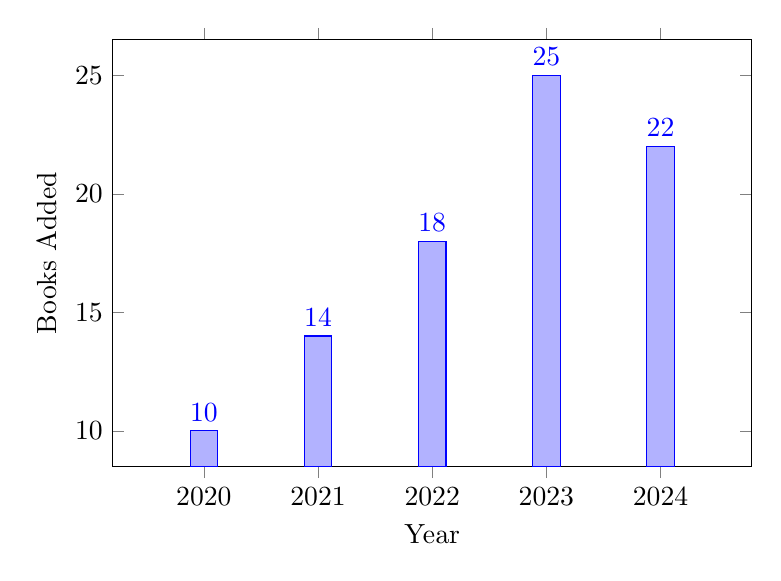
\begin{tikzpicture}
    \begin{axis}[
      ybar,
      enlarge x limits=0.2,
      width=0.8\textwidth,
      height=7cm,
      ylabel={Books Added},
      xlabel={Year},
      symbolic x coords={2020,2021,2022,2023,2024},
      xtick=data,
      nodes near coords,
      nodes near coords align={vertical}
    ]
    \addplot coordinates {(2020,10) (2021,14) (2022,18) (2023,25) (2024,22)};
    \end{axis}
  \end{tikzpicture}
  \caption{Sample visualization: Books added per year (example data)}
\end{figure}

\section{Conclusion}
The Library Management System effectively addresses the problem of manual book record handling by providing a simple yet functional digital solution. The modular code allows future integration with databases and front-end systems, and Git version control ensures collaborative scalability.

\section{Future Improvements}
To enhance this project further, the following steps can be taken:
\begin{itemize}
  \item Implement a persistent storage system using JSON, CSV, or SQL.
  \item Add a user authentication system for librarians.
  \item Create a graphical interface using Tkinter or a web framework like Flask.
  \item Integrate automated testing and CI/CD workflows.
  \item Visualize data dynamically using libraries such as Matplotlib or Plotly.
\end{itemize}

\end{document}